% Data flow diagram
% Author: David Fokkema
\documentclass{article}
\usepackage{tikz}
\usetikzlibrary{shapes,arrows}
\usepackage{pdflscape}
\usepackage[papersize={15cm, 8.7cm}, text={14cm, 9.2cm}]{geometry}
\usetikzlibrary{decorations.text}
\usepackage{xcolor}
\usepackage{graphicx}
% \selectcolormodel{gray}

\begin{document}
\thispagestyle{empty}
%\begin{landscape}
\begin{center}
\begin{tikzpicture}[node distance=2cm,
  font=\sffamily,
  every matrix/.style={ampersand replacement=\&,column sep=0.8cm,row
sep=0.4cm,font=\scriptsize},
  sent/.style={draw,thick,rectangle,fill=green!20,font=\scriptsize},
  word/.style={draw,thick,ellipse,fill=blue!20},
  lf/.style={draw,thick,rectangle,fill=yellow!20,font=\scriptsize},
  word/.style={draw,thick,ellipse,fill=blue!20},
  figg/.style={thick,rectangle,fill=white!20,font=\scriptsize},
  word/.style={draw,thick,ellipse,fill=blue!20},
  mediator/.style={draw,thick,circle},
  entityType/.style={draw,thick,rounded corners,fill=yellow!20,inner
sep=.3cm,font=\scriptsize},
  model/.style={draw,thick,rounded corners,fill=violet!20,inner
sep=.3cm,font=\scriptsize},
  mathType/.style={draw,thick,diamond,fill=red!20,font=\sc\scriptsize},
  mediatorToEntity/.style={->,>=stealth',shorten
>=1pt,semithick,black,sloped,above,font=\sffamily\scriptsize},
  typeToEntity/.style={->,>=stealth',shorten
>=1pt,semithick,black,sloped,above,font=\sffamily\scriptsize},
  wordToEntity/.style={-,>=stealth',shorten >=1pt,ultra
thick,dotted,blue,sloped,above,font=\sffamily\scriptsize},
  entityToMath/.style={->,>=stealth',shorten >=1pt,ultra
thick,dashed,violet,sloped,above,font=\sffamily\scriptsize},
  ans/.style={draw,thick,rectangle},
  every node/.style={align=center,distance=2cm}]

   \node (webcorpus) [word, xshift=-2cm] {\large Sentence};
   \node (sentence) [sent,right of=webcorpus, xshift=2.8cm,fill=white] {\large Dependency \\ \large Tree};
   \node (lf) [lf,right of=sentence, xshift=4cm,font=\tiny] {\large General-purpose \\ \large Logical Form};
   \node (ug) [figg,below of=lf,yshift=-1cm] {\hspace{-1.5cm} 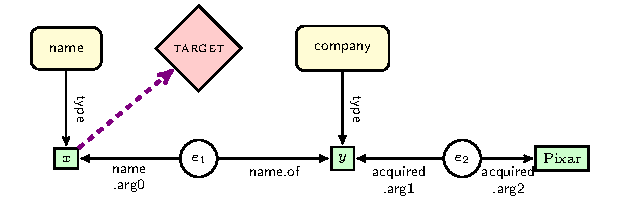
\includegraphics[scale=0.5,trim=0em 0em 0em 0em,clip=true]{transitive_ungrounded_mismatch} \\ \large Ungrounded Graph};
   \node (db) [figg,left of=ug,xshift=-3cm,yshift=-1cm] {\includegraphics[scale=0.3]{db}};
   \node (gg) [figg,left of=ug,xshift=-7cm] {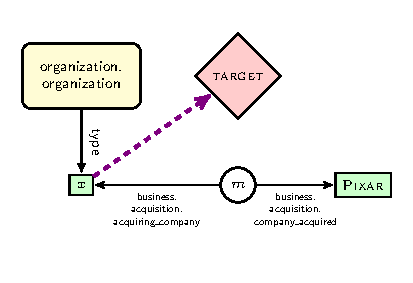
\includegraphics[scale=0.5,trim=1em 2em 1em 0em,clip=true]{transitive_grounded}\\ \large Freebase Graph};
   \node (mod) [model,below of=db,yshift=-0.7cm] {\small Denotation-based \\ \small Learning Model};
   \node (quest) [sent,left of=mod,xshift=-2.1cm] {Who acquired Pixar?};
   \node (ans) [ans,right of=mod,xshift=2cm] {\{Disney\}};
   
   \draw [mediatorToEntity] (webcorpus) -- node[magenta] {\hspace{-0.2cm} \large Dependency \\ \large Parser} (sentence);
   \draw [mediatorToEntity] (sentence) -- node[blue] {\large UD \large to Logic} (lf);
   \draw [mediatorToEntity] ([xshift=-1cm]ug.west) -- node[red] {\Large Graph Matching}  (gg);
   \draw [entityToMath] (lf) -- (ug);
   \draw [mediatorToEntity] (ug) -- (mod);
   \draw [mediatorToEntity] (gg) -- (mod);
   \draw [mediatorToEntity] (db) -- (mod);
   \draw [mediatorToEntity] (quest) -- (mod);
   \draw [mediatorToEntity] (mod) -- (ans);
\end{tikzpicture} 
\end{center}

\end{document}
